\documentclass[../main.tex]{subfiles}
\graphicspath{{\subfix{../images/}}}

\setcounter{secnumdepth}{0}
\begin{document}

\section{3. domácí úlohy}

\subsection{1a)}
\subsubsection*{Zadání}
Buď $G=(V,E)$ $k$-regulární bipartitní graf s částmi $L$ a $R$. Dokažte, že $|L|=|R|$.

\subsubsection*{Řešení}

Počet hran vycházejících z $L$ je zřejmě $k |L|$, počet hran vycházejících z $R$, je zřejmě $|k|R$.

Je zřejmé, že se oba tyto výrazy musí rovnat (jedná se o 2 různé způsoby jak spočíst všechny hrany v grafu), proto tedy $|L| = |R|$
\qed


\subsection{1b)}
\subsubsection*{Zadání}
Nalezněte, až na isomorfismus, všechny bipartitní grafy $G$, jejichž doplněk $\bar{G}$ je též bipartitní.

\subsubsection*{Řešení}

Po provedení doplňku se z $L$ a $R$ stanou úplné podgrafy. Vezměme tedy třeba úplný podgraf $\bar{L}$, 
pokud je $|L|>2$ určitě by v něm existoval lichý cyklus. 
Protože podgraf bipartitního grafu musí být také bipartitní dostáváme, že
$|L|, |R| \leq 2$. 

Z tohoto plyne, že aby pro  graf $G=(V,E)$ platilo, že jeho doplněk je bipartitní tak pak $|V|\leq 4$.

Navíc také platí, že mezi každou trojicí vrcholů musí být buď 1 nebo 2 hrany. V opačném případě existuje v grafu nebo jeho doplňku lichý cyklus.

Z toho plyne že $G$ nemůže být prázdný/úplný pro $|V|\geq 3$.

Pro případ $|V| = 4$ tedy dostáváme následující grafy:

Jako množinu vrcholů vezměme $[4]$. 

BÚNO (jinak by šlo pouze o izomorfismus) má graf  hranu $\{1,2\}$. 
Mezi vrcholy $2,3,4$ ale není žádná hrana, kvůli předchozímu tvrzení musíme mezi nimi jednu hranu přidat.
Máme 2 možnosti (kvůli izomorfismu) buď přidáme hranu $\{2,3\}$ nebo $\{3,4\}$  $(\star)$.

Pro případ $\{2,3\}$, ale opět chybí hrana mezi $1,3,4$, hranu $\{1,3\}$ přidat nemůžeme, vznikl by cyklus o délce 3. Proto přidáme 
hranu například $\{3,4\}$ (druhá možnost je opět izomorfní s touto). Doplněk tohoto grafu je pak izomorfní se sebou samým. Rozdělení které existuje je $L = \{1,3\}, R = \{2,4\}$.

Nakonec bychom k tomuto grafu ještě mohli přidat hranu $\{4,1\}$, vznikl by cyklus, doplněk tohoto grafu by byl izomorfní s grafem s hranami  $\{1,2\}, \{3,4\}$ (tímto jsme se dostali k $(\star)$, navíc z grafu s hranami $\{1,2\}, \{3,4\}$ dostaneme přidáním libovolné hrany graf isomorfní s předchozím případem).
Tento graf je i se svým doplňkem opět bipartitní, volme například $L = \{1,3\}, R = \{2,4\}$.


Případ $|V| = 3$:

Jako množinu vrcholů vezměme $[3]$. 

BÚNO má graf  hranu $\{1,2\}$. Přidáním další hrany dostaneme jeho doplněk a oba tyto grafy jsou bipartitní.

Případ $|V| = 2$:

Prázdný graf je zřejmě bipartitní, jeho doplněk je $G=([2], {1,2})$ je také.

Případ $|V| = 1,0$:

Oba dva tyto degenerované případy jsou bipartitní a jsou doplňkem sebe sama. 

Na obrázku můžeme vidět všechny grafy s jejich doplňky (bez degenerovaných případů). 
Obarvení určuje rozdělení do $L$ a $R$

\begin{figure}[!h]
    \centering
    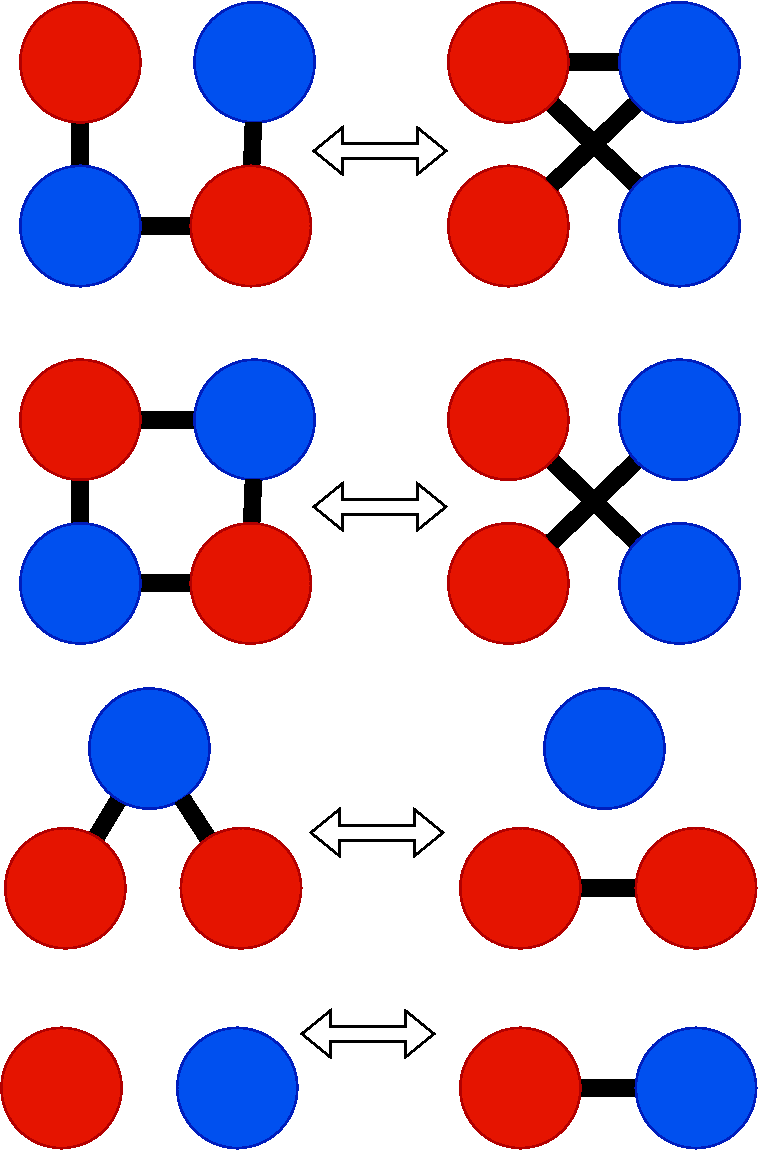
\includegraphics[height=\linewidth]{images/BipartiteComplement.pdf}
    \caption*{Všechny bipartitní grafy jejichž doplněk je také bipartitní}
\end{figure}






\subsection{2)}
\subsubsection*{Zadání}
Pro graf $G=(V,E)$ označme průměrem $G$ maximální délku nejkratší cesty mezi nějakými dvěma vrcholy, tzn. $\max_{u,v\in V} \text{dist}_{G}(u,v)$. Dokažte, že má-li graf průměr alespoň 4, tak jeho doplněk má průměr nejvýše 2.

\subsubsection*{Řešení}


\subsection{3)}
\subsubsection*{Zadání}
Pro graf $G=(V,E)$ označme $g(G)$ délku nejkratšího cyklu, který $G$ obsahuje; pokud je $G$ acycklický, definujeme $g(G)\coloneq \infty$.
Poznamenejme, že parametru $g(G)$ se také říká obvod grafu.

Buď $d\geq 3$ a $r\geq 2$ pevné a $G=(V,E)$ libovolný $d$-regulární graf. Dokažte
\begin{enumerate}
    \item Je-li $g(G)=2r$, tak  potom $|V| \geq \frac{2(d-1)^r -2}{d-2}$
    \item Je-li $g(G) = 2r + 1$ tak potom $|V|\geq \frac{d(d-1)^r -2}{d-2}$
\end{enumerate}

\subsubsection*{Řešení}


\subsection{4)}
Připomeňme, že pro graf $G=(V,E)$ nazveme hranu $e\in E$ mostem, jestliže podgraf $(V,E\setminus\{e\})$ má více komponent souvislosti než $G$.\\
Analogicky nazveme vrchol $v\in V$ artikulací, jestliže indukovaný podgraf množinou $V\setminus{v}$ má více komponent souvislosti než $G$.

\subsection{4a)}
\subsubsection*{Zadání}
Dokažte, že každý $2k$- regulární graf neobsahuje most.



\subsubsection*{Řešení}


\subsection{4b)}
\subsubsection*{Zadání}
Dokažte, že každý $k$-regulární bipartitní graf neobsahuje artikulaci.

\subsubsection*{Řešení}


\subsection{5a)}
\subsubsection*{Zadání}
Buď $G=(V,E)$ neprázdný graf a buď $d \coloneq \frac{|E|}{|V|}$. Dokažte, že $G$ obsahuje indukovaný podgraf $H$ splňující $\delta(H) > d$.

(Nápověda: zkuste z $G$ postupně odebírat vrcholy stupně nejvýše $d$.)

\subsubsection*{Řešení}


\subsection{5b)}
\subsubsection*{Zadání}
Pro každé přirozené $d\geq 1$ a každé $\varepsilon\in(0,1)$ zkonstruujte graf $G_{d,\varepsilon}= (V,E)$
takový, že splňuje $\frac{|E|}{|V|} > d - \varepsilon$ a zároveň $\delta(H)\leq d$ pro každý podgraf $H \subseteq G_{d,\varepsilon}$.


\subsubsection*{Řešení}

\end{document}